\documentclass{article}
\usepackage{enumitem}
\usepackage{listings}
\usepackage{color}
\usepackage{amsmath}
\usepackage{hyperref}
\usepackage{graphicx}
\usepackage{animate}

\graphicspath{ {./} }

\definecolor{codegreen}{rgb}{0,0.6,0}
\definecolor{codegray}{rgb}{0.5,0.5,0.5}
\definecolor{codepurple}{rgb}{0.58,0,0.82}
\definecolor{backcolour}{rgb}{0.95,0.95,0.92}
 
\setlist[itemize]{font=\tiny\bfseries}

\begin{document}

	\title{MMC laboratory01}
	\author{Terman Emil FAF161}
	\maketitle

	\newpage
	\section{1. Hyperbolic Tangent}
    After implementing this exercise, I noticed that for big numbers, the other 2
given formulas, fail, even though the result is almost 1. That's because, exp(n)
or sinh(n) or cosh(n), for $>$ 700 (about so), are huge numbers - so huge, they
don't fit in their given memory.
\newline
    To resolve this problem, I use the lambert formula:
\newline    
    $tanh(x) = \frac{x}{
        1 + \frac{x ^ 2}{
            3 + \frac{x ^ 2}{
                5 + ...
            }
        }
    }$
\newline
    So that I don't have to depend on huge numbers. To make the results more
precises, I store the numbers as fraction. In this way, the results are very
exact, but the it takes considerably more time to compute.
\newline
    To emphasize the exactness of fractions, I also used floating points. As a
result, I recive a tiny, but yet visible error.
\newline
    So, if I'd build a program for some rocket science, I would be aware that
some numbers, like 0.1, even though it seems a small number, it's actually an
periodic sequence in binary representation, and since we can't store infinite
sequences - we have to chop the value, making that little error that led to "The Explosion of the Ariane 5"

    \newpage
    \section{2. Some Code}
    In computer, not all real numbers can be stored as floating point numbers.
That's because, there are some numbers that their binary representation may be
too big to fit in the given memory for floats, in which case - the number is
either choped or rounded, producing an error. An example of such a thing is
0.1 whith its binary representation: 0.0001100110011... Well, ofcourse the error
is not big, unless it's multiplied to a big number, let's say 1000 or 10000. To
resolve such cases, we could use Fractions or Fixed point numbers.
\newline
    $>$ Fractions: instead of storing 0.1, we can store it as 1/10, in which
case we avoid the choping or rounding of the number.
\newline
    $>$ Fixed point numbers: are less prcise, but much more consistent, because
the numbers are stored inside an integer.
\newline
    Conclusion: never use floats for additive operations (float += float) on
big scales

    \newpage
    \section{3. Integrals}
    Deomnstration:
    \newline
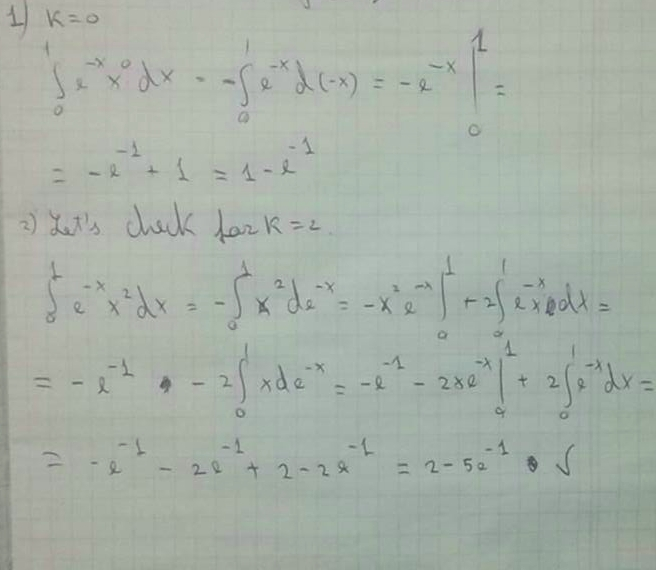
\includegraphics[scale=0.6]{ex3_demonstration}
    \newline
	\par To avoid any error depending on additions or multiplications, I calculated
the result in integers, then I substitued e with its value.
        
My program's results:

	k)  $<built in integral> : <recursive(float)> (<recursive(explicit)>)$
	\begin{itemize}
		\setlength\itemsep{-5pt}
		
		\item {\small 0)  0.632121 : 0.632121 (1 - 1/e)}
		\item {\small 1)  0.264241 : 0.264241 (1 - 2/e)}
		\item {\small 2)  0.160603 : 0.160603 (2 - 5/e)}
		\newline...
		\item {\small 11)  0.033195 : 0.033195 (39916800 - 108505112/e)}
		\item {\small 12)  0.030463 : 0.030463 (479001600 - 1302061345/e)}
		\item {\small 13)  0.028145 : 0.028145 (6227020800 - 16926797486/e)}
		\item {\small 14)  0.026154 : 0.026154 (87178291200 - 236975164805/e)}
		\item {\small 15)  0.024424 : 0.024414 (1307674368000 - 3554627472076/e)}
		\item {\small 16)  0.022909 : 0.023438 (20922789888000 - 56874039553217/e)}
		\item {\small 17)  0.021570 : 0.000000 (355687428096000 - 966858672404690/e)}
		\item {\small 18)  0.020378 : 0.000000 (6402373705728000 - 17403456103284421/e)}
		\item {\small 19)  0.019311 : 0.000000 (121645100408832000 - 330665665962404000/e)}
		\item {\small 20)  0.018350 : 0.000000 (2432902008176640000 - 6613313319248080001/e)}

		\item {\small 21)  0.017480 : 0.000000 (51090942171709440000 - 138879579704209680022/e)}
		
		\item {\small 22)  0.016689 : 0.000000 (1124000727777607680000 - 3055350753492612960485/e)}
		
		\item {\small 23)  0.015966 : 0.000000 (25852016738884976640000 - 70273067330330098091156/e)}
		
		\item {\small 24)  0.015303 : 0.000000 (620448401733239439360000 - 1686553615927922354187745/e)}
		
		\item {\small 25)  0.014693 : -2147483648.000000 (15511210043330985984000000 - 42163840398198058854693626/e)}
	\end{itemize}

	\par Let's say for a given k, the result is of the form: a - b/e

	\begin{itemize}
    	\item As k grows, so does a and b. When k reaches 25, b becomes a big number, Taking in consideration that e is irrational, meaning that its value is choped, then it means that it generates a certain error. Multiplied that with 42163840398198058854693626, the error becomes much bigger, therefore, creating erroneous values.

    	\item When two numbers are nearly equal and we subtract them, then we suffer a Loss of Significance error in the calculation. It usually happens when one gets too few significant digits in substraction of two numbers very close to each other.
	\end{itemize}
	\par Let's say we have the number:
	\begin{enumerate}
		\item \begin{center}
			1.2345678
		\end{center}

		and another number, very close to the first one:
		
		\item \begin{center}
			1.2344444
		\end{center}
		
		When the difference is calculated, we recive:
		
		\item \begin{center}
			0.0001234
		\end{center}
	\end{enumerate}
	\par The first 2 numbers have 8 significant digits and the substraction of these numbers lead to a number with 4 significant digits, making a \textbf{Loss of Significance}. The first 2 numbers have a realtive round off error of about $10^{-8}$, but the result has a round off error of $10 ^ {-4}$, which is a much bigger error.
	\par In the case with the integral, we experience a clear loss of significance starting from k = 17. The difference between \textit{a} and \textit{b/e}, apparently has too few significant digits exceeding the limit of representable numbers, so the computer rounds the result to 0.
	\par For k = 25, the result would've been 0 aswell, if not for the error of \textit{e}.
    \newpage
    \section{4. Fractal}

    	\begin{center}
			
\includegraphics[scale=0.7]{fractal}
		\end{center}
    
		\par Using the Julia Sets, we can create a very beautiful, infinite and chaotic image.

		\par This formula can describe the chaos: because it's infinite, we could say that everything has a fractal form.

		\par The branching of tracheal tubes, the leaves in trees, the veins in a hand, tiny oxygene molecule, or the DNA molecule - all these can be described as fractals.

		\par Some people say that the spreading of the universe is fractal. Others try to predict the stock market using fractals.
		
		\par In conclusion: Fractals are not just some pretty pictures, but a whole new way of thinking about the universe

		\begin{center}
			\par \textbf{Check out the gifs}
		\end{center}
\end{document}
